\documentclass[10pt]{beamer}
\usefonttheme{professionalfonts}
%\usetheme{CambridgeUS}
%
% Choose how your presentation looks.
%
% For more themes, color themes and font themes, see:
% http://deic.uab.es/~iblanes/beamer_gallery/index_by_theme.html
%
\mode<presentation>
{
  \usetheme{default}      % or try Darmstadt, Madrid, Warsaw, ...
  \usecolortheme{beaver} % or try albatross, beaver, crane, ...
  \usefonttheme{default}  % or try serif, structurebold, ...
  \setbeamertemplate{navigation symbols}{}
  \setbeamertemplate{caption}[numbered]
} 

\usepackage[english]{babel}
\usepackage[utf8x]{inputenc}
\usepackage{tikz}
\usepackage{pgfplots}
\usepackage{array}  % for table column M
\usepackage{makecell} % to break line within a cell
\usepackage{verbatim}
\usepackage{graphicx}
\usepackage{epstopdf}
\usepackage{amsfonts}
\usepackage{xcolor}
%\captionsetup{compatibility=false}
%\usepackage{dsfont}
\usepackage[absolute,overlay]{textpos}
\usetikzlibrary{calc}
\usetikzlibrary{pgfplots.fillbetween, backgrounds}
\usetikzlibrary{positioning}
\usetikzlibrary{arrows}
\usetikzlibrary{pgfplots.groupplots}
\usetikzlibrary{arrows.meta}
\usetikzlibrary{plotmarks}

\usepgfplotslibrary{groupplots}
\pgfplotsset{compat=newest} 
%\pgfplotsset{plot coordinates/math parser=false}

\usepackage{hyperref}
\hypersetup{
    colorlinks=true,
    linkcolor=blue,
    filecolor=magenta,      
    urlcolor=cyan,
}

\definecolor{matlabcomment}{RGB}{34,139,34}

\pgfmathdeclarefunction{gauss}{1}{%
	\pgfmathparse{1/(sqrt(2*pi))*exp(-((#1)^2)/2)}%
}

\pgfmathdeclarefunction{laplacian}{2}{%
	\pgfmathparse{1/(#2*2)*exp(-(abs(x-#1))/(#2))}%
}

\pgfmathdeclarefunction{pretty_func}{1}{%
	\pgfmathparse{cos(deg(#1/2)) - sin(deg(#1)) + cos(deg(#1/2)-45) - sin(deg(#1/4)-154)}%
}

\pgfplotsset{
	dirac/.style={
		mark=triangle*,
		mark options={scale=2},
		ycomb,
		scatter,
		visualization depends on={y/abs(y)-1 \as \sign},
		scatter/@pre marker code/.code={\scope[rotate=90*\sign,yshift=-2pt]}
	}
}

\tikzset{
	invisible/.style={opacity=0},
	visible on/.style={alt={#1{}{invisible}}},
	alt/.code args={<#1>#2#3}{%
		\alt<#1>{\pgfkeysalso{#2}}{\pgfkeysalso{#3}} % \pgfkeysalso doesn't change the path
	},
}

\newcommand\PlotSampledSpectrum[4]{%
	\def\fs{#2}%
	\def\fmax{#3}%
	\def\ros{#4}%
	\input{#1}%
}

\pgfmathdeclarefunction{invgauss}{2}{%
	\pgfmathparse{sqrt(-2*ln(#1))*cos(deg(2*pi*#2))}%
}

\tikzset{
	declare function={
		sinc(\x) = (and(\x!=0, 1) * (sin(deg(pi*\x))/(pi*\x)) +
		(and(\x==0, 1) * 1);
	}
}

\DeclareMathOperator{\E}{\mathbb{E}} % expectation

\newcolumntype{M}[1]{>{\centering\arraybackslash}m{#1}}

\definecolor{blue2}{RGB}{51, 105, 232}  
\definecolor{red2}{RGB}{213, 15, 37}  
\definecolor{green2}{RGB}{0, 153, 37}  
\definecolor{green3}{rgb}{0.1922, 0.6392, 0.3294}% 
\definecolor{yellow2}{RGB}{238, 178, 17} 
\definecolor{gray2}{RGB}{102, 102, 102}
\definecolor{orange2}{RGB}{230, 85, 13}

% Qualitative pallete set1 from www.ColorBrewer.org
\definecolor{Qred}{RGB}{228,26,28}
\definecolor{Qblue}{RGB}{55,126,184}
\definecolor{Qgreen}{RGB}{77,175,74}
\definecolor{Qpurple}{RGB}{152,78,163}
\definecolor{Qorange}{RGB}{255,127,0}
\definecolor{Qyellow}{RGB}{255,255,51}
\definecolor{Qbrown}{RGB}{166,86,40}
\definecolor{Qpink}{RGB}{247,129,191}
\definecolor{Qgray}{RGB}{153,153,153}

\newcommand\PlotGaussianCF[4]{%
	\def\sig{#2}%
	\def\ws{#3}%
	\def\cap{#4}
	\input{#1}%
}

\title[EE 264]{Quantization}
\author{Jose Krause Perin}
\institute{Stanford University}
\date{July 13, 2017}

\begin{document}

\begin{frame}
  \titlepage
\end{frame}

%
\begin{frame}{Announcements}
	\begin{itemize}
		\item Homework \#2 due today
		\item Homework \#3 will be released today and it is due next Thursday
	\end{itemize}
\end{frame}


%
\section{Outline}
\begin{frame}{Outline}
\begin{itemize}
	\item Probabilistic interpretation of quantization
	\item Linear noise model
	\item Quantization noise shaping
\end{itemize}
\end{frame}

%
\section{Quantization in DSP}
\begin{frame}{Practice and theory}
\begin{block}{In practice}
	\begin{center}
		\resizebox{\linewidth}{!}{\def\layersep{1.5cm}
\def\outsep{0.7cm}
\def\dy{1.25}

\begin{tikzpicture}[->, >=stealth, shorten >= 0pt, draw=black!50, node distance=\layersep, font=\sffamily]
    \tikzstyle{node}=[circle,fill=black,minimum size=2pt,inner sep=0pt]
    \tikzstyle{block}=[draw=black,rectangle,fill=none,minimum size=1.5cm, inner sep=0pt]
    \tikzstyle{annot} = []

	\node[node] (xc) at (0, -\dy cm) {};
    \node[block] (ADC) at (1*\layersep, -\dy cm) {ADC};
    \node[block, text width = 2.5cm, align= center] (DSP) at (3*\layersep, -\dy cm) {Digital Signal Processor};
    \node[block] (DAC) at (5*\layersep, -\dy cm) {DAC};
	\coordinate (yc) at (6*\layersep, -\dy cm) {};
	
	\coordinate (mid1) at ($(ADC.east)!0.5!(DSP.west)$) {};
	\coordinate (mid2) at ($(DSP.east)!0.5!(DAC.west)$) {};
		
    \path (xc) edge (ADC);
    \path (ADC) edge (DSP);
    \path (DSP) edge (DAC);
    \path (DAC) edge (yc);
    
    \node[above = 0.5mm of mid1] {$x[n]$};
    \node[above = 0.5mm of mid2] {$y[n]$};
    \node[left = 0mm of xc, text width = 1cm, align=center] {$x_c(t)$};
    \node[right = 0mm of yc, text width = 1cm, align=center] {$y_c(t)$}; 
    

\end{tikzpicture}}
	\end{center}
\end{block}

\begin{block}{DSP theory}
	\begin{center}
		\resizebox{\linewidth}{!}{\def\layersep{2cm}
\def\outsep{0.7cm}
\def\dy{1.25}

\begin{tikzpicture}[->, >=stealth, shorten >= 0pt, draw=black!50, node distance=\layersep, font=\sffamily]
    \tikzstyle{node}=[circle,fill=black,minimum size=2pt,inner sep=0pt]
    \tikzstyle{block}=[draw=black,rectangle,fill=none,minimum size=1.5cm, inner sep=0pt]
    \tikzstyle{annot} = []

	\node[node] (xc) at (0, -\dy cm) {};
    \node[block] (ADC) at (1*\layersep, -\dy cm) {C-to-D};
    \node[block, text width = 2cm, align= center] (DSP) at (3*\layersep, -\dy cm) {LTI \\ System};
    \node[block] (DAC) at (5*\layersep, -\dy cm) {D-to-C};
	\coordinate (yc) at (6*\layersep, -\dy cm) {};
	
	\coordinate (mid1) at ($(ADC.east)!0.5!(DSP.west)$) {};
	\coordinate (mid2) at ($(DSP.east)!0.5!(DAC.west)$) {};
		
    \path (xc) edge (ADC);
    \path (ADC) edge (DSP);
    \path (DSP) edge (DAC);
    \path (DAC) edge (yc);
    
    \node[above = 0.5mm of mid1] {$x[n]$};
    \node[below = 0.5mm of mid1] {$X(e^{j\omega})$};
    \node[above = 0.5mm of mid2] {$y[n]$};
    \node[below = 0.5mm of mid2] {$Y(e^{j\omega})$};
    \node[above = 0mm of xc, text width = 1cm, align=center] {$x_c(t)$};
    \node[below = 0mm of xc, text width = 1cm, align=center] {$X_c(j\Omega)$};
    \node[above = 0mm of yc, text width = 1cm, align=center] {$y_r(t)$}; 
    \node[below = 0mm of yc, text width = 1cm, align=center] {$Y_r(j\Omega)$};
    \node at ($(DSP.south)-(0, 0.25cm)$) {$h[n] \leftrightarrow H(e^{j\omega})$};
\end{tikzpicture}}
	\end{center}

	\textbf{Problem:} This simplified model does not account for \textbf{quantization} (today's lecture) and \textbf{finite precision arithmetic} (lecture 8)
\end{block}
\end{frame}

%
\begin{frame}{Including quantization}
	\begin{block}{Analog-to-digital converter}
		A more realistic model
		\begin{center}
		\resizebox{0.9\linewidth}{!}{
			\begin{tikzpicture}[->, >=stealth, shorten >= 0pt, draw=black!50, node distance=2.75cm, font=\sffamily]
				\tikzstyle{node}=[circle,fill=black,minimum size=2pt,inner sep=0pt]
				\tikzstyle{block}=[draw=black,rectangle,fill=none,minimum size=1.5cm, inner sep=0pt]
				
				\node[node] (xc) {};
				\node[block, right=1cm of xc] (CTD) {C-to-D};
				\node[block, right of=CTD, text width = 2cm, align= center] (Q) {Quantizer};
				\node[block, right of=Q] (coder) {Coder};
				\coordinate[right=1.5cm of coder] (yc) {};
				
				\coordinate (mid1) at ($(CTD.east)!0.5!(Q.west)$) {};
				\coordinate (mid2) at ($(Q.east)!0.5!(coder.west)$) {};
				
				\path (xc) edge (CTD);
				\path (CTD) edge (Q);
				\path (Q) edge (coder);
				\path (coder) edge (yc);
				
				\node[above = 0.5mm of mid1] {$x[n]$};
				\node[above = 0.5mm of mid2] {$x_Q[n]$};
				\node[above = 0mm of xc, text width = 1cm, align=center] {$x_c(t)$};
				\node[above = 0mm of yc, align=center] {$x_B[n]$}; 
				\node[below = 0mm of yc, text width = 2.5cm, align=center] {Binary \\ representation}; 
				
				\node[align=center] at ($(CTD.south)-(0, 0.4cm)$) {Sampling \\ $T$};
				\node[align=center, text width=4cm] at ($(Q.south)-(0, 1.1cm)$) {Analog-to-digital converter};
				
				\draw[dashed] ($(CTD.south west)-(0.25, 0.8)$) rectangle ($(coder.north east)+(0.25, 0.3)$) {};
				
			\end{tikzpicture}
		}
		\end{center}
	\end{block}
\end{frame}

%
\begin{frame}{Quantizer}
	\begin{columns}[t]
		\begin{column}{0.5\textwidth}
			\textbf{Mid-tread} uniform quantizer
			\resizebox{\textwidth}{!}{\begin{tikzpicture}
	\tikzstyle{node}=[circle,draw=black!50,fill=black,minimum size=2pt,inner sep=0pt]
	\tikzstyle{block}=[draw=black,rectangle,fill=none,minimum size=1cm, inner sep=0pt]
	\begin{axis}[
		axis lines*=middle,
		enlargelimits = false, clip=false,
		ymin=-4, ymax=5,
		xmin=-5, xmax=5,
		axis line style={->,>=stealth},
		xlabel={$x$},
		ylabel={$Q(x)$},
		yticklabel style = {yshift=0.2cm},
		xticklabel style = {yshift=-0.1cm},
		every axis x label/.style={
			at={(ticklabel* cs:1)},
			anchor=west,
		},
		every axis y label/.style={
			at={(ticklabel* cs:1)},
			anchor=south,
		},
		ytick={-4, -3,-2, 1, 2, 3},
		yticklabels={$-4\Delta$, $-3\Delta$, $-2\Delta$, $\Delta$, $2\Delta$, $3\Delta$},
		xtick={-4.5,...,4.5},
		xticklabels={$-\frac{9\Delta}{2}$, $-\frac{7\Delta}{2}$, $-\frac{5\Delta}{2}$, $-\frac{3\Delta}{2}$, $-\frac{\Delta}{2}$, $\frac{\Delta}{2}$, $\frac{3\Delta}{2}$, $\frac{5\Delta}{2}$, $\frac{7\Delta}{2}$, $\frac{9\Delta}{2}$},
		every outer y axis line/.append style={white!15!black},
		every y tick label/.append style={font=\color{white!15!black}},
		legend style={draw=white!15!black,fill=white,legend cell align=left}]			
		\addplot[line width=1pt] coordinates {(0, 0) (1/2, 0) (1/2, 1) (3/2, 1) (3/2, 2) (5/2, 2) (5/2, 3) (5, 3)};
		\addplot[line width=1pt] coordinates {(0, 0) (-1/2, 0) (-1/2, -1) (-3/2, -1) (-3/2, -2) (-5/2, -2) (-5/2, -3) (-7/2, -3) (-7/2, -4) (-5, -4)};
		\addplot[dashed, black!20, line width=1pt, domain=-4:4, samples=2] {x};
		
		\draw[black!10, fill=black!10] (axis cs: -6, 4) rectangle (axis cs: -1, 2) {};
		\node[node] (xc) at (axis cs: -5.5, 3) {};
		\node[block, right=0.75cm of xc, text width = 1cm, align= center] (Q) {$Q$};
		\coordinate[right=0.75cm of Q] (yc) {};
		
		\path[->, >=stealth, shorten >= 0pt, draw=black!50] (xc) edge (Q);
		\path[->, >=stealth, shorten >= 0pt, draw=black!50] (Q) edge (yc);
		
		\node[above = 0mm of xc, text width = 1cm, align=center] {$x[n]$};
		\node[above = 0mm of yc, align=center] {$x_Q[n]$}; 
		
		\draw[<->, >=stealth, blue2, line width=2pt] (axis cs: -4.5, 0.25) -- (axis cs: 3.5, 0.25) {};
		\node at (axis cs: 2.5, 0.75) {\color{blue2} $\Delta X$}; 
	\end{axis}
\end{tikzpicture}}
		\end{column}
	
		\begin{column}{0.5\textwidth}
			\textbf{Mid-rise} uniform quantizer
			\resizebox{\textwidth}{!}{\begin{tikzpicture}
			\tikzstyle{node}=[circle,draw=black!50,fill=black,minimum size=2pt,inner sep=0pt]
			\tikzstyle{block}=[draw=black,rectangle,fill=none,minimum size=1cm, inner sep=0pt]
			\begin{axis}[
			axis lines*=middle,
			enlargelimits = false, clip=false,
			ymin=-4, ymax=5,
			xmin=-5, xmax=5,
			axis line style={->,>=stealth},
			xlabel={$x[n]$},
			ylabel={$Q(x)$},
			yticklabel style = {yshift=0.2cm},
			xticklabel style = {yshift=-0.1cm},
			every axis x label/.style={
				at={(ticklabel* cs:1)},
				anchor=west,
			},
			every axis y label/.style={
				at={(ticklabel* cs:1)},
				anchor=south,
			},
			xtick={-4,..., 4},
			xticklabels={$-4\Delta$, $-3\Delta$, $-2\Delta$, $-\Delta$, 0, $\Delta$, $2\Delta$, $3\Delta$, $4\Delta$},
			ytick={-4, -3,-2, 1, 2, 3, 4},
			yticklabels={$-4\Delta$, $-3\Delta$, $-2\Delta$, $\Delta$, $2\Delta$, $3\Delta$, $4\Delta$},
			every outer y axis line/.append style={white!15!black},
			every y tick label/.append style={font=\color{white!15!black}},
			legend style={draw=white!15!black,fill=white,legend cell align=left}]			
			\addplot[line width=1pt] coordinates {(0, -1) (0, 1) (1, 1) (1, 2) (2, 2) (2, 3) (3, 3) (3, 4) (4, 4) (5, 4)};
			\addplot[line width=1pt] coordinates {(0, -1) (-1, -1) (-1, -2) (-2, -2) (-2, -3) (-3, -3) (-3, -4) (-4, -4) (-5, -4)};
			\addplot[dashed, black!20, line width=1pt, domain=-4:4, samples=2] {x};
			
			\draw[black!10, fill=black!10] (axis cs: -6, 4) rectangle (axis cs: -1, 2) {};
			\node[node] (xc) at (axis cs: -5.5, 3) {};
			\node[block, right=0.75cm of xc, text width = 1cm, align= center] (Q) {$Q$};
			\coordinate[right=0.75cm of Q] (yc) {};
			
			\path[->, >=stealth, shorten >= 0pt, draw=black!50] (xc) edge (Q);
			\path[->, >=stealth, shorten >= 0pt, draw=black!50] (Q) edge (yc);
			
			\node[above = 0mm of xc, text width = 1cm, align=center] {$x[n]$};
			\node[above = 0mm of yc, align=center] {$x_Q[n]$}; 
			
			\draw[<->, >=stealth, blue2, line width=2pt] (axis cs: -4, 0.5) -- (axis cs: 4, 0.5) {};
			\node at (axis cs: 2.5, 1) {\color{blue2} $\Delta X$}; 
			\end{axis}
			\end{tikzpicture}}
		\end{column}
	\end{columns}
	\begin{center}
		
	\end{center}
	
	\textbf{Terminology}
	\begin{itemize}
		\item The quantizer has $B$ bits of \textbf{resolution}
		\item $\Delta X$ is the \textbf{dynamic range}
		\item $\Delta$ is the \textbf{step size}
	\end{itemize}

	\begin{equation}
	\Delta = \frac{\Delta X}{2^{B}} \label{eq:Delta}
	\end{equation}
\end{frame}

%
\begin{frame}{Example of quantization}
\begin{center}
	\resizebox{0.6\textwidth}{!}{\begin{tikzpicture} 
\begin{axis}[
axis lines*=middle,
enlargelimits = true,
ymin=-4.5, ymax=4.5,
xmin=0, xmax=7,
axis line style={->,>=stealth},
xlabel={$n$},
yticklabel style = {yshift=0.2cm},
xticklabel style = {yshift=-0.1cm},
every axis x label/.style={
    at={(ticklabel* cs:1)},
    anchor=north,
},
every axis y label/.style={
    at={(ticklabel* cs:1)},
    anchor=south,
},
xtick=\empty,
ytick={-4,...,4},
yticklabels={$-4\Delta$,$-3\Delta$, $-2\Delta$, $-\Delta$, 0, $\Delta$, $2\Delta$, $3\Delta$, $4\Delta$},
every outer x axis line/.append style={white!15!black},
every x tick label/.append style={font=\color{white!15!black}},
ymajorgrids,
every outer y axis line/.append style={white!15!black},
every y tick label/.append style={font=\color{white!15!black}},
legend style={draw=white!15!black,fill=white,legend cell align=left, at={(axis cs: 9, 5)}}]

\addplot[black!20, domain=0:7, samples=31, forget plot] {4.7*cos(1.1*deg(x)-135)};
\addplot[ycomb, mark=*, domain=0:7, samples=8] {4.7*cos(1.1*deg(x)-135)}; \addlegendentry{$x[n]$};
\only<2-|handout:1>{
\addplot[ycomb, red, mark=*, domain=0:7, samples=8] {round(4.5*cos(1.1*deg(x)-135))}; \addlegendentry{$x_Q[n] = Q(x[n])$};

\node[draw=orange, circle, minimum size=0.75cm, line width=1pt] at (axis cs: 2, 4.3) {};
\node[draw=orange, circle, minimum size=0.75cm, line width=1pt] (c2) at (axis cs: 5, -4.3) {};
\node at (axis cs: 6.25, -4.7) {\color{orange} clipping};
}
\end{axis}
\end{tikzpicture}
}
\end{center}

\onslide<2-|handout:1>{
Quantization error:
\begin{align*}
e[n] = x[n] - Q(x[n]) = x[n] - x_Q[n]
\end{align*}
Note that the quantization error is bounded $-\Delta/2 \leq e[n] \leq \Delta/2$.
}

\onslide<3-|handout:1>{
The quantization error is deterministic but hard to analyze, so we'll treat it as noise (random process).
}

\end{frame}

%
\begin{frame}{Quantization of a sinusoid}
	\only<1-3|handout:1>{Using a 3-bit quantizer}
	\only<4-6|handout:2>{Using an 8-bit quantizer}
	\begin{center}
		\resizebox{0.75\textwidth}{!}{\def\H{0.3\textwidth}
\def\W{\textwidth}

\begin{tikzpicture}
\onslide<1-3|handout:1>{
\begin{axis}[
name=plot1,
axis lines*=middle,
enlargelimits = true,
width=\W,
height=\H,
clip=true,
scale only axis,
axis line style={->,>=stealth},
xlabel={ $n$},
ylabel={ $x[n]$},
every axis x label/.style={
	at={(ticklabel* cs:1)},
	xshift=-0.2cm,
	anchor=north,
},
every axis y label/.style={
	at={(ticklabel* cs:1)},
	xshift=0.5cm,
	yshift=-0.35cm,
	anchor=south,
},
every outer x axis line/.append style={white!15!black},
every x tick label/.append style={font=\color{white!15!black}},
xmin=0.00, xmax=7.00,
ymin=-5.00, ymax=5.00,
ytick=\empty,
xtick=\empty,
yticklabel=\empty,
xmajorgrids,
ymajorgrids,
every outer y axis line/.append style={white!15!black},
every y tick label/.append style={font=\color{white!15!black}},
legend style={draw=white!15!black,fill=white,legend cell align=left}]
\addplot [ycomb, black, mark=*, mark options={scale=0.75, fill=white}, line width=1.5pt, domain=0:7, samples=61, forget plot] {4.5*cos(deg(x))};
\end{axis}
}

\onslide<2-3|handout:1>{
	\begin{axis}[
		name=plot2,
		at=(plot1.below south east), anchor=above north east,
		axis lines*=middle,
		enlargelimits = true,
		width=\W,
		height=\H,
		clip=true,
		scale only axis,
		axis line style={->,>=stealth},
		xlabel={ $n$},
		ylabel={ $x_Q[n]$},
		every axis x label/.style={
			at={(ticklabel* cs:1)},
			xshift=-0.2cm,
			anchor=north,
		},
		every axis y label/.style={
			at={(ticklabel* cs:1)},
			xshift=0.6cm,
			yshift=-0.35cm,
			anchor=south,
		},
		every outer x axis line/.append style={white!15!black},
		every x tick label/.append style={font=\color{white!15!black}},
		xmin=0.00, xmax=7.00,
		ymin=-5.00, ymax=5.00,
		ytick=\empty,
		xtick=\empty,
		yticklabel=\empty,
		xmajorgrids,
		ymajorgrids,
		every outer y axis line/.append style={white!15!black},
		every y tick label/.append style={font=\color{white!15!black}},
		legend style={draw=white!15!black,fill=white,legend cell align=left}]
		\addplot [ycomb, black, mark=*, mark options={scale=0.75, fill=white}, line width=1.5pt, domain=0:7, samples=61, forget plot] {round(4.25*cos(deg(x)))};
	\end{axis}
}

\onslide<3|handout:1>{
	\begin{axis}[
	name=plot3,
	at=(plot2.below south east), anchor=above north east,
	axis lines*=middle,
	enlargelimits = true,
	width=\W,
	height=\H,
	clip=true,
	scale only axis,
	axis line style={->,>=stealth},
	xlabel={ $n$},
	ylabel={ $e[n] = x[n] - x_Q[n]$},
	every axis x label/.style={
		at={(ticklabel* cs:1)},
		xshift=-0.2cm,
		anchor=north,
	},
	every axis y label/.style={
		at={(ticklabel* cs:1)},
		xshift=1.7cm,
		yshift=-0.35cm,
		anchor=south,
	},
	every outer x axis line/.append style={white!15!black},
	every x tick label/.append style={font=\color{white!15!black}},
	xmin=0.00, xmax=7.00,
	ymin=-1.00, ymax=1.00,
	ytick=\empty,
	xtick=\empty,
	yticklabel=\empty,
	xmajorgrids,
	ymajorgrids,
	every outer y axis line/.append style={white!15!black},
	every y tick label/.append style={font=\color{white!15!black}},
	legend style={draw=white!15!black,fill=white,legend cell align=left}]
	\addplot [ycomb, black, mark=*, mark options={scale=0.75, fill=white}, line width=1.5pt, domain=0:7, samples=61, forget plot] {4.25*cos(deg(x)) - round(4.25*cos(deg(x)))};
	\end{axis}
}

%% 8-bit quantizer
\onslide<4-|handout:2>{
	\begin{axis}[
	name=plot1,
	axis lines*=middle,
	enlargelimits = true,
	width=\W,
	height=\H,
	clip=true,
	scale only axis,
	axis line style={->,>=stealth},
	xlabel={ $n$},
	ylabel={ $x[n]$},
	every axis x label/.style={
		at={(ticklabel* cs:1)},
		xshift=-0.2cm,
		anchor=north,
	},
	every axis y label/.style={
		at={(ticklabel* cs:1)},
		xshift=0.5cm,
		yshift=-0.35cm,
		anchor=south,
	},
	every outer x axis line/.append style={white!15!black},
	every x tick label/.append style={font=\color{white!15!black}},
	xmin=0.00, xmax=7.00,
	ymin=-17.7778, ymax=17.7778,
	ytick=\empty,
	xtick=\empty,
	yticklabel=\empty,
	xmajorgrids,
	ymajorgrids,
	every outer y axis line/.append style={white!15!black},
	every y tick label/.append style={font=\color{white!15!black}},
	legend style={draw=white!15!black,fill=white,legend cell align=left}]
	\addplot [ycomb, black, mark=*, mark options={scale=0.75, fill=white}, line width=1.5pt, domain=0:7, samples=61, forget plot] {16*cos(deg(x))};
	\end{axis}
}

\onslide<5-|handout:2>{
	\begin{axis}[
	name=plot2,
	at=(plot1.below south east), anchor=above north east,
	axis lines*=middle,
	enlargelimits = true,
	width=\W,
	height=\H,
	clip=true,
	scale only axis,
	axis line style={->,>=stealth},
	xlabel={ $n$},
	ylabel={ $x_Q[n]$},
	every axis x label/.style={
		at={(ticklabel* cs:1)},
		xshift=-0.2cm,
		anchor=north,
	},
	every axis y label/.style={
		at={(ticklabel* cs:1)},
		xshift=0.6cm,
		yshift=-0.35cm,
		anchor=south,
	},
	every outer x axis line/.append style={white!15!black},
	every x tick label/.append style={font=\color{white!15!black}},
	xmin=0.00, xmax=7.00,
	ymin=-17.7778, ymax=17.7778,
	ytick=\empty,
	xtick=\empty,
	yticklabel=\empty,
	xmajorgrids,
	ymajorgrids,
	every outer y axis line/.append style={white!15!black},
	every y tick label/.append style={font=\color{white!15!black}},
	legend style={draw=white!15!black,fill=white,legend cell align=left}]
	\addplot [ycomb, black, mark=*, mark options={scale=0.75, fill=white}, line width=1.5pt, domain=0:7, samples=61, forget plot] {round(16*cos(deg(x)))};
	\end{axis}
}

\onslide<6-|handout:2>{
	\begin{axis}[
	name=plot3,
	at=(plot2.below south east), anchor=above north east,
	axis lines*=middle,
	enlargelimits = true,
	width=\W,
	height=\H,
	clip=true,
	scale only axis,
	axis line style={->,>=stealth},
	xlabel={ $n$},
	ylabel={ $e[n] = x[n] - x_Q[n]$},
	every axis x label/.style={
		at={(ticklabel* cs:1)},
		xshift=-0.2cm,
		anchor=north,
	},
	every axis y label/.style={
		at={(ticklabel* cs:1)},
		xshift=1.7cm,
		yshift=-0.35cm,
		anchor=south,
	},
	every outer x axis line/.append style={white!15!black},
	every x tick label/.append style={font=\color{white!15!black}},
	xmin=0.00, xmax=7.00,
	ymin=-1.00, ymax=1.00,
	ytick=\empty,
	xtick=\empty,
	yticklabel=\empty,
	xmajorgrids,
	ymajorgrids,
	every outer y axis line/.append style={white!15!black},
	every y tick label/.append style={font=\color{white!15!black}},
	legend style={draw=white!15!black,fill=white,legend cell align=left}]
	\addplot [ycomb, black, mark=*, mark options={scale=0.75, fill=white}, line width=1.5pt, domain=0:7, samples=61, forget plot] {16*cos(deg(x)) - round(16*cos(deg(x)))};
	\end{axis}
}
\end{tikzpicture}}
	\end{center}
\end{frame}

%
\section{Probabilistic Interpretation of Quantization}
\begin{frame}{Probability distribution of the output of a quantizer}
\textbf{Question:} what's the probability density function (PDF) $p_{x_Q}(x)$ of the quantizer output $x_Q[n] \sim p_{x_Q}(x)$ when the input signal $x[n]$ has PDF $x[n] \sim p_{x}(x)$?
\begin{center}
	\resizebox{0.75\textwidth}{!}{\begin{tikzpicture}
\begin{axis}[
name=plot1,
width=\textwidth,
height=0.5\textwidth,
axis lines*=middle,
enlargelimits = upper, clip=true,
scale only axis,
axis line style={->,>=stealth},
xlabel={\Large $x$},
ylabel={\Large $p_x(x)$},
every axis x label/.style={
	at={(ticklabel* cs:1)},
	xshift=-0.2cm,
	anchor=north,
},
every axis y label/.style={
	at={(ticklabel* cs:0.9)},
	xshift=0.7cm,
	anchor=south,
},
every outer x axis line/.append style={white!15!black},
every x tick label/.append style={font=\color{white!15!black}},
xmin=-3.00, xmax=3.4,
ymin=0, ymax=0.5,
ytick=\empty,
xtick={-2.5, -1.5, -0.5, 0.5, 1.5, 2.5},
xticklabels={\large $-\frac{5\Delta}{2}$, \large$-\frac{3\Delta}{2}$, \large$-\frac{\Delta}{2}$,\large $\frac{\Delta}{2}$, \large$\frac{3\Delta}{2}$, \large$\frac{5\Delta}{2}$},
xmajorgrids,
ymajorgrids,
every outer y axis line/.append style={white!15!black},
every y tick label/.append style={font=\color{white!15!black}},
legend style={draw=white!15!black,fill=white,legend cell align=left, at={(axis cs: 3, 0.25)}}]

\addplot [name path=g, smooth, black, line width=1.5pt, domain=-5:5, samples=51, forget plot] {gauss(x)};
\path[name path=axis1] (axis cs:-0.5,0) -- (axis cs:0.5,0);

\addplot [
thick,
color=black,
fill=black, 
fill opacity=0.10,
forget plot,
]
fill between[
of=g and axis1,
soft clip={domain=-0.5:0.5},
];

\node[black, fill=black!10, minimum size=1cm] at (axis cs: 1.75, 0.45) {\Large $\mathrm{Pr}(-\Delta/2 \leq x \leq \Delta/2)$};

\only<3-|handout:1>{
\addplot [dirac, line width=1.5pt] coordinates {(-2, 0.05) (-1, 0.15) (0, 0.3) (1, 0.15) (2, 0.05)}; \addlegendentry{\Large $p_{x_Q}(x)$};
}

\only<2-|handout:1>{
	\addplot [dirac, line width=1.5pt, forget plot] coordinates {(0, 0.3)};
}
\end{axis}
\end{tikzpicture}
}
\end{center}

\onslide<4|handout:1>{
The PDF of $x_Q[n] \sim p_{x_Q}(x)$ is formed by impulses at the quantization levels. The area of any given impulse is equal to the area under $p_x(x)$ in the quantization interval corresponding to that impulse. In the example of the figure, the area of the impulse at the origin is equal to the highlighted area under $p_x(x)$.
}
\end{frame}

%
\begin{frame}{Area sampling}
We can view $p_{x_Q}(x)$ as samples of the area of $p_x(x)$ under quantization intervals. This form of sampling is called \textbf{area sampling}.

\begin{equation*}
p_{x_Q}(x) = \underbrace{(p_x(x) \ast r(x))}_{\text{\normalsize area calculation}}\overbrace{\cdot s(x)}^{\text{\normalsize sampling}},
\end{equation*}
where 
\begin{equation*}
r(x) = \begin{cases}
\frac{1}{\Delta}, & -\frac{\Delta}{2} \leq x \leq \frac{\Delta}{2} \\
0, & \text{otherwise}
\end{cases} \tag{rectangular window of area 1}
\end{equation*}

\begin{equation*}
s(x) = \sum_{n = -\infty}^{\infty} \delta(x - n\Delta) \tag{impulse train}
\end{equation*}
The period of the impulse train (\textit{sampling period}) is $\Delta$

\textbf{Interesting:} although quantization is an nonlinear operation on the signal, it is a linear operation on that signal PDF, since area sampling is linear.
\end{frame}

%
\begin{frame}{Area sampling: graphically}
\begin{center}
	\resizebox{0.9\textwidth}{!}{\begin{tikzpicture}
\onslide<1-|handout:1>{
\begin{axis}[
	name=plot1,
	axis lines*=middle,
	enlargelimits = upper, clip=true,
	scale only axis,
	width=\textwidth,
	height=0.2\textwidth,
	ymin=0, ymax=0.5,
	xmin=-5, xmax=5,
	axis line style={->,>=stealth},
	xlabel={\small $x$},
	ylabel={\small $p_x(x)$},
	every axis x label/.style={
		at={(ticklabel* cs:1)},
		anchor=north,
	},
	every axis y label/.style={
		at={(ticklabel* cs:0.8)},
		anchor=south,
		xshift=0.6cm,
	},
	xtick={-3,...,3},
	xticklabels={$-3\Delta$,$-2\Delta$, $-\Delta$, 0, $\Delta$, $2\Delta$, $3\Delta$},
	ytick=\empty,
	every outer y axis line/.append style={white!15!black},
	every y tick label/.append style={font=\color{white!15!black}},
	legend style={draw=white!15!black,fill=white,legend cell align=left}]
	\addplot[smooth, line width=1pt, domain=-5:5, samples=31] {gauss(x)};
\end{axis}
}

\onslide<2-|handout:1>{
\begin{axis}[
	name=plot2,
	at=(plot1.below south east), anchor=above north east,
	axis lines*=middle,
	enlargelimits = upper, clip=true,
	scale only axis,
	width=\textwidth,
	height=0.2\textwidth,
	ymin=0, ymax=1.5,
	xmin=-5, xmax=5,
	axis line style={->,>=stealth},
	xlabel={\small $x$},
	ylabel={\small $r(x)$},
	every axis x label/.style={
		at={(ticklabel* cs:1)},
		anchor=north,
	},
	every axis y label/.style={
		at={(ticklabel* cs:0.8)},
		anchor=south,
		xshift=0.6cm,
	},
	xtick={-0.5, 0.5},
	ytick=1,
	yticklabels={$\frac{1}{\Delta}$},
	yticklabel style={yshift=0.3cm},
	xticklabels={$-\frac{\Delta}{2}$, $\frac{\Delta}{2}$}, 
	every outer y axis line/.append style={white!15!black},
	every y tick label/.append style={font=\color{white!15!black}},
	legend style={draw=white!15!black,fill=white,legend cell align=left}]
	\addplot[solid, line width=1pt] coordinates {(-5, 0) (-1/2, 0) (-1/2, 1) (1/2, 1) (1/2, 0) (5, 0)};
\end{axis}
}

\onslide<3|handout:0>{
	\begin{axis}[
	name=plot3,
	at=(plot2.below south east), anchor=above north east,
	axis lines*=middle,
	enlargelimits = upper, clip=true,
	scale only axis,
	width=\textwidth,
	height=0.2\textwidth,
	ymin=0, ymax=0.5,
	xmin=-5, xmax=5,
	axis line style={->,>=stealth},
	xlabel={\small $x$},
	ylabel={\small $p_x(x) \ast r(x)$},
	every axis x label/.style={
		at={(ticklabel* cs:1)},
		anchor=north,
	},
	every axis y label/.style={
		at={(ticklabel* cs:0.8)},
		anchor=south,
		xshift=1cm,
	},
	xtick=\empty,
	ytick=\empty,
	every outer y axis line/.append style={white!15!black},
	every y tick label/.append style={font=\color{white!15!black}},
	legend style={draw=white!15!black,fill=white,legend cell align=left}]
\addplot [smooth, line width=1pt, forget plot]
table[row sep=crcr]{
	-5 3.1178e-06 \\
-4.8 8.1063e-06 \\
-4.6 1.9895e-05 \\
-4.4 4.6364e-05 \\
-4.2 0.00010396 \\
-4 0.00022431 \\
-3.8 0.00046577 \\
-3.6 0.0009308 \\
-3.4 0.0017904 \\
-3.2 0.0033151 \\
-3 0.0059093 \\
-2.8 0.010142 \\
-2.6 0.01676 \\
-2.4 0.026672 \\
-2.2 0.040879 \\
-2 0.060346 \\
-1.8 0.085813 \\
-1.6 0.11756 \\
-1.4 0.15515 \\
-1.2 0.1973 \\
-1 0.24176 \\
-0.8 0.28547 \\
-0.6 0.32484 \\
-0.4 0.35623 \\
-0.2 0.3765 \\
0 0.38351 \\
0.2 0.3765 \\
0.4 0.35623 \\
0.6 0.32484 \\
0.8 0.28547 \\
1 0.24176 \\
1.2 0.1973 \\
1.4 0.15515 \\
1.6 0.11756 \\
1.8 0.085813 \\
2 0.060346 \\
2.2 0.040879 \\
2.4 0.026672 \\
2.6 0.01676 \\
2.8 0.010142 \\
3 0.0059093 \\
3.2 0.0033151 \\
3.4 0.0017904 \\
3.6 0.0009308 \\
3.8 0.00046577 \\
4 0.00022431 \\
4.2 0.00010396 \\
4.4 4.6364e-05 \\
4.6 1.9895e-05 \\
4.8 8.1063e-06 \\
5 3.1178e-06 \\
};

\end{axis}
}


\onslide<4-|handout:1>{
	\begin{axis}[
	name=plot3,
	at=(plot2.below south east), anchor=above north east,
	axis lines*=middle,
	enlargelimits = upper, clip=true,
	scale only axis,
	width=\textwidth,
	height=0.2\textwidth,
	ymin=0, ymax=0.5,
	xmin=-5, xmax=5,
	axis line style={->,>=stealth},
	xlabel={\small $x$},
	ylabel={\small $p_{x_Q}(x) = (p_x(x) \ast r(x))\cdot s(x)$},
	every axis x label/.style={
		at={(ticklabel* cs:1)},
		anchor=north,
	},
	every axis y label/.style={
		at={(ticklabel* cs:0.8)},
		anchor=south,
		xshift=2.3cm,
	},
	xtick={-3,...,3},
	xticklabels={$-3\Delta$,$-2\Delta$, $-\Delta$, 0, $\Delta$, $2\Delta$, $3\Delta$},
	ytick=\empty,
	every outer y axis line/.append style={white!15!black},
	every y tick label/.append style={font=\color{white!15!black}},
	legend style={draw=white!15!black,fill=white,legend cell align=left}]
	\addplot [smooth, black!20, line width=1pt, forget plot]
	table[row sep=crcr]{
		-5 3.1178e-06 \\
		-4.8 8.1063e-06 \\
		-4.6 1.9895e-05 \\
		-4.4 4.6364e-05 \\
		-4.2 0.00010396 \\
		-4 0.00022431 \\
		-3.8 0.00046577 \\
		-3.6 0.0009308 \\
		-3.4 0.0017904 \\
		-3.2 0.0033151 \\
		-3 0.0059093 \\
		-2.8 0.010142 \\
		-2.6 0.01676 \\
		-2.4 0.026672 \\
		-2.2 0.040879 \\
		-2 0.060346 \\
		-1.8 0.085813 \\
		-1.6 0.11756 \\
		-1.4 0.15515 \\
		-1.2 0.1973 \\
		-1 0.24176 \\
		-0.8 0.28547 \\
		-0.6 0.32484 \\
		-0.4 0.35623 \\
		-0.2 0.3765 \\
		0 0.38351 \\
		0.2 0.3765 \\
		0.4 0.35623 \\
		0.6 0.32484 \\
		0.8 0.28547 \\
		1 0.24176 \\
		1.2 0.1973 \\
		1.4 0.15515 \\
		1.6 0.11756 \\
		1.8 0.085813 \\
		2 0.060346 \\
		2.2 0.040879 \\
		2.4 0.026672 \\
		2.6 0.01676 \\
		2.8 0.010142 \\
		3 0.0059093 \\
		3.2 0.0033151 \\
		3.4 0.0017904 \\
		3.6 0.0009308 \\
		3.8 0.00046577 \\
		4 0.00022431 \\
		4.2 0.00010396 \\
		4.4 4.6364e-05 \\
		4.6 1.9895e-05 \\
		4.8 8.1063e-06 \\
		5 3.1178e-06 \\
	};
	
	\addplot [dirac, line width=1pt, forget plot]
	table[row sep=crcr]{
		-2 0.053991 \\
		-1 0.24197 \\
		0 0.39894 \\
		1 0.24197 \\
		2 0.053991 \\
	};
	\end{axis}
}

\end{tikzpicture}
}
\end{center}	
\end{frame}

%
\begin{frame}{Random variables and convolution}
The area sampling interpretation of quantization gives us a simple equation for the PDF of $x_Q[n]$:
\begin{equation*}
p_{x_Q}(x) = \underbrace{(p_x(x) \ast r(x))}_{\text{\normalsize area calculation}}\overbrace{\cdot s(x)}^{\text{\normalsize sampling}},
\end{equation*}

\pause
\textbf{Another interpretation:} in probability theory, we use convolution to calculate the PDF of the \textbf{sum of two independent random variables}:

\begin{equation*}
Z = X + Y \Longrightarrow p_Z = p_X \ast p_Y
\end{equation*}

\pause
Applying to our problem:

\begin{equation*}
\tilde{x}_Q[n] = x[n] + q[n] \Longrightarrow p_{\tilde{x}_Q}(x) = \underbrace{(p_x(x) \ast r(x))}_{\text{\normalsize area calculation}}
\end{equation*}
where $q[n]$ is a random variable independent of $x[n]$ and with PDF $p_q(x) = r(x)$. Therefore, $q$ is an \textbf{uniform random variable} ($q\sim\mathcal{U}[-\Delta/2, \Delta/2]$).
\end{frame}

%
\begin{frame}
Comparing with the definition of quantization error:
\begin{align*}
x_Q[n] &= x[n] - e[n] \tag{from definition of quantization error} \\
\tilde{x}_Q[n] &= x[n] + q[n] \tag{from probabilistic interpreation of area sampling}
\end{align*}

The equations for $x_Q[n]$ and $\tilde{x}_Q[n]$ are very similar, but there's an important difference. The PDF $p_{x_Q}(x)$ is formed by \textbf{sampling} $p_{\tilde{x}_Q}(x)$.

\pause
\begin{center}
	\resizebox{0.55\textwidth}{!}{\begin{tikzpicture}
\begin{axis}[
	axis lines*=middle,
	enlargelimits = upper, clip=true,
	scale only axis,
	width=0.8\textwidth,
	height=0.4\textwidth,
	ymin=0, ymax=0.4,
	xmin=-4, xmax=4,
	axis line style={->,>=stealth},
	xlabel={\Large $x$},
	ylabel={\huge $p_{x_Q}(x) = \underbrace{(p_x(x) \ast r(x))}_{\Large p_{\tilde{x}_Q}(x)}\cdot s(x)$},
	every axis x label/.style={
		at={(ticklabel* cs:1)},
		anchor=north,
	},
	every axis y label/.style={
		at={(ticklabel* cs:0.8)},
		anchor=south,
		xshift=2.3cm,
	},
	xtick={-3,...,3},
	xticklabels={$-3\Delta$,$-2\Delta$, $-\Delta$, 0, $\Delta$, $2\Delta$, $3\Delta$},
	ytick=\empty,
	every outer y axis line/.append style={white!15!black},
	every y tick label/.append style={font=\color{white!15!black}},
	legend style={draw=white!15!black,fill=white,legend cell align=left}]
	\addplot [smooth, black!20, line width=1pt, forget plot]
	table[row sep=crcr]{
		-5 3.1178e-06 \\
		-4.8 8.1063e-06 \\
		-4.6 1.9895e-05 \\
		-4.4 4.6364e-05 \\
		-4.2 0.00010396 \\
		-4 0.00022431 \\
		-3.8 0.00046577 \\
		-3.6 0.0009308 \\
		-3.4 0.0017904 \\
		-3.2 0.0033151 \\
		-3 0.0059093 \\
		-2.8 0.010142 \\
		-2.6 0.01676 \\
		-2.4 0.026672 \\
		-2.2 0.040879 \\
		-2 0.060346 \\
		-1.8 0.085813 \\
		-1.6 0.11756 \\
		-1.4 0.15515 \\
		-1.2 0.1973 \\
		-1 0.24176 \\
		-0.8 0.28547 \\
		-0.6 0.32484 \\
		-0.4 0.35623 \\
		-0.2 0.3765 \\
		0 0.38351 \\
		0.2 0.3765 \\
		0.4 0.35623 \\
		0.6 0.32484 \\
		0.8 0.28547 \\
		1 0.24176 \\
		1.2 0.1973 \\
		1.4 0.15515 \\
		1.6 0.11756 \\
		1.8 0.085813 \\
		2 0.060346 \\
		2.2 0.040879 \\
		2.4 0.026672 \\
		2.6 0.01676 \\
		2.8 0.010142 \\
		3 0.0059093 \\
		3.2 0.0033151 \\
		3.4 0.0017904 \\
		3.6 0.0009308 \\
		3.8 0.00046577 \\
		4 0.00022431 \\
		4.2 0.00010396 \\
		4.4 4.6364e-05 \\
		4.6 1.9895e-05 \\
		4.8 8.1063e-06 \\
		5 3.1178e-06 \\
	} node[pos=0.65, black, pin={[pin edge={black, thick}]40:{\color{black} \Large $p_{\tilde{x}_Q}(x)$}}, inner sep=0pt] {};

	
	\addplot [dirac, line width=1pt, forget plot]
	table[row sep=crcr]{
		-2 0.053991 \\
		-1 0.24197 \\
		0 0.39894 \\
		1 0.24197 \\
		2 0.053991 \\
	};
\end{axis}
\end{tikzpicture}}
\end{center}

\pause
If the sampled PDF ($p_{x_Q}(x)$) perfectly describes $p_{\tilde{x}_Q}(x)$, we can say that quantization error is perfectly described by an uniform random process.

\pause 
\textbf{Question:}  under what conditions can we perfectly reconstruct $p_{\tilde{x}_Q}(x)$ from its samples? \\
\end{frame}

%
\begin{frame}{Revisiting the Shannon-Nyquist theorem}
	Recall that the \textbf{Shannon-Nyquist theorem} guarantees that we can perfectly recover a signal from its samples if two conditions are met:
	\begin{enumerate}
		\item \textbf{No aliasing; spectrum replicas do not overlap}
		\item Use ideal reconstruction filter (ideal lowpass filter)
	\end{enumerate}
	\pause
	\begin{block}{Conditions for no aliasing}
		\begin{enumerate}
			\item The \textbf{characteristic function} (Fourier transform) of the area-sampled input PDF must satisfy: 
			\begin{equation*}
				\Phi_{p_{x_Q}}(j\theta) = \mathcal{F}\{p_{x_Q}(x)\} = 0, |\theta| > \theta_N
			\end{equation*}
			This is analogous to the condition of a signal being \textit{band-limited}.
			\item\pause The \textit{sampling frequency} $\theta_s$ must be such that $\theta_s > 2\theta_N$.
			
			In this context, $\theta_s = 2\pi/\Delta$, and the quantization interval $\Delta$ is equivalent to the \textit{sampling period} (period of the impulse train).
		\end{enumerate}
	\end{block}
\end{frame}

%
\begin{frame}<beamer:0|handout:1>
Additional comments
\begin{itemize}
	\item When we used the Shannon-Nyquist theorem for sampling a continuous-time signal, we said that we can use an anti-aliasing filter to minimize aliasing, but we could not use the ideal lowpass filter, as it is unfeasible.
	\item In this discussion on quantization, we just want theoretical assurance that we can reconstruct the PDF from its samples. Therefore, for this purpose, we can use the ideal lowpass filter.
	\item On the other hand, we cannot guarantee that there won't be aliasing, as many probability distributions are not \textit{band-limited}.
\end{itemize}
\end{frame}

%
\begin{frame}
	\textbf{Conclusion:} if the conditions for no aliasing are met, we can perfectly reconstruct the original PDF from its samples, and therefore, quantization noise can be \underline{perfectly modeled} as an uniform random process.
	
	\pause
	\textbf{Bad news:} the conditions for no aliasing are generally not met in practice. \textbf{Example:} Gaussian distribution. The characteristic function of the Gaussian distribution is a Gaussian function. The Gaussian function is not \textit{band-limited}, as it is always non-zero.
	
	\pause
	\textbf{How can we mitigate aliasing?}
	\begin{enumerate}
		\item Anti-aliasing filter? This would be equivalent to modify the PDF of the input signal. But what would it do the signal?
		\item Oversampling $\implies$ shorter sampling period ($\Delta$) $\implies$ finer quantization
	\end{enumerate}
\end{frame}

% 
\begin{frame}{Example for the Gaussian input distribution}
	\begin{itemize}
		\item A zero-mean Gaussian distributed signal with variance $\sigma^2$ is quantized with quantization resolution \tikz[baseline]{\node[fill=black!10,anchor=base] {$\Delta = 2.1\sigma$};}
		\item Overlap of spectrum replicas results in \underline{significant aliasing}
		\item The estimated quantization noise PDF differs from the uniform distribution
	\end{itemize}
	
	\begin{columns}[t]
		\begin{column}{0.5\textwidth}
			Fourier transform of sampled PDF
				\begin{center}
					\resizebox{\textwidth}{!}{\PlotGaussianCF{figs/aliased_gaussian_cf.tex}{1}{2.9920}{$\Delta = 2.1\sigma$}}
				\end{center}
		\end{column}
			\begin{column}{0.5\textwidth}
			Estimated quantization noise PDF
			\begin{center}
					\resizebox{0.9\textwidth}{!}{\begin{tikzpicture}
\begin{axis}[
xmin=-1, xmax=1,
axis lines*=center,
every axis y label/.style={at=(current axis.above origin),anchor=south},
every axis x label/.style={at=(current axis.right of origin),anchor=west},
%height=5cm, width=8cm,
xtick=\empty,
ytick=\empty,
xticklabel=\empty,
ymin=0,
ymax=0.6,
yticklabel style={yshift=0.5cm, xshift=0.8cm},
ylabel={\Large $p_{e}(e)$},
xlabel={\Large $e$},
enlargelimits=false, clip=true, axis on top,
grid = major,
axis line style={->,>=stealth, shorten >= -10pt},
every axis x label/.style={
	at={(ticklabel* cs:1)},
	yshift=0.2cm,
	xshift=0.5cm,
	anchor=north,
},
every axis y label/.style={
	at={(ticklabel* cs:1)},
	anchor=south,
	xshift=0.3cm,
	yshift=0.3cm,
},
xtick={-1, 1},
ytick=0.5,
yticklabels={\Large $\frac{1}{\Delta}$},
xticklabels={\Large$-\frac{\Delta}{2}$, \Large $\frac{\Delta}{2}$},
]
\addplot[black, ybar interval, fill=black!20, mark=no] 
table[row sep=crcr]{
	-1.029 0.4681 \\
	-0.987 0.46555 \\
	-0.945 0.46698 \\
	-0.903 0.46238 \\
	-0.861 0.46662 \\
	-0.819 0.46579 \\
	-0.777 0.46467 \\
	-0.735 0.46533 \\
	-0.693 0.4645 \\
	-0.651 0.47183 \\
	-0.609 0.473 \\
	-0.567 0.47052 \\
	-0.525 0.47769 \\
	-0.483 0.47964 \\
	-0.441 0.4845 \\
	-0.399 0.47945 \\
	-0.357 0.4756 \\
	-0.315 0.48581 \\
	-0.273 0.48245 \\
	-0.231 0.48512 \\
	-0.189 0.48455 \\
	-0.147 0.48971 \\
	-0.105 0.49229 \\
	-0.062999 0.48376 \\
	-0.020999 0.48714 \\
	0.021001 0.48774 \\
	0.063 0.48517 \\
	0.105 0.48286 \\
	0.147 0.48495 \\
	0.189 0.49255 \\
	0.231 0.49062 \\
	0.273 0.48731 \\
	0.315 0.47883 \\
	0.357 0.48307 \\
	0.399 0.4764 \\
	0.441 0.47657 \\
	0.483 0.47974 \\
	0.525 0.47679 \\
	0.567 0.47707 \\
	0.609 0.47186 \\
	0.651 0.47183 \\
	0.693 0.46886 \\
	0.735 0.4711 \\
	0.777 0.46469 \\
	0.819 0.47233 \\
	0.861 0.47057 \\
	0.903 0.46924 \\
	0.945 0.46526 \\
	0.987 0.46519 \\
	1.029 0.46595 \\
};
\addplot[black, domain=-1:1, samples=2] {0.5};
\end{axis}
\end{tikzpicture}}
			\end{center}
			\end{column}
	\end{columns}
\end{frame}

%
\begin{frame}{Example for the Gaussian input distribution}
\begin{itemize}
	\item A zero-mean Gaussian distributed signal with variance $\sigma^2$ is quantized with quantization resolution \tikz[baseline]{\node[fill=black!10,anchor=base] {$\Delta = \sigma$};}
	\item Spectrum replicas are sufficiently apart; \underline{aliasing is negligible}
	\item The estimated quantization noise PDF agrees well with the uniform distribution
\end{itemize}

\begin{columns}[t]
	\begin{column}{0.5\textwidth}
		Fourier transform of sampled PDF
		\begin{center}
			\resizebox{\textwidth}{!}{\PlotGaussianCF{figs/aliased_gaussian_cf.tex}{1}{6.2832}{$\Delta = \sigma$}}
		\end{center}
	\end{column}
	\begin{column}{0.5\textwidth}
		Estimated quantization noise PDF
		\begin{center}
			\resizebox{0.9\textwidth}{!}{\begin{tikzpicture}
\begin{axis}[
xmin=-0.5,
xmax=0.5,
axis lines*=center,
every axis y label/.style={at=(current axis.above origin),anchor=south},
every axis x label/.style={at=(current axis.right of origin),anchor=west},
%height=5cm, width=8cm,
xtick=\empty,
ytick=\empty,
xticklabel=\empty,
ymin=0,
ymax=1.2,
yticklabel style = {xshift=0.4cm, yshift=-0.2cm},
ylabel={\Large $p_{e}(e)$},
xlabel={\Large  $e$},
enlargelimits=false, clip=true, axis on top,
grid = major,
axis line style={->,>=stealth, shorten >= -10pt},
every axis x label/.style={
	at={(ticklabel* cs:1)},
	yshift=0.2cm,
	xshift=0.5cm,
	anchor=north,
},
every axis y label/.style={
	at={(ticklabel* cs:1)},
	anchor=south,
	xshift=0.3cm,
	yshift=0.3cm,
},
xtick={-0.5, 0.5},
ytick=1,
yticklabel style={yshift=0.6cm, xshift=0.3cm},
yticklabels={\Large $\frac{1}{\Delta}$},
xticklabels={\Large $-\frac{\Delta}{2}$, \Large $\frac{\Delta}{2}$},
]
\addplot[black, ybar interval, fill=black!20, mark=no] 
table[row sep=crcr]{
	-0.49 0.9955 \\
	-0.47 0.992 \\
	-0.45 0.9993 \\
	-0.43 0.99245 \\
	-0.41 1.0013 \\
	-0.39 1.0004 \\
	-0.37 1.0103 \\
	-0.35 0.99475 \\
	-0.33 0.99625 \\
	-0.31 0.99365 \\
	-0.29 1.0048 \\
	-0.27 0.98945 \\
	-0.25 0.9939 \\
	-0.23 1.0035 \\
	-0.21 1.0031 \\
	-0.19 1.0093 \\
	-0.17 0.9976 \\
	-0.15 0.9988 \\
	-0.13 0.99205 \\
	-0.11 1.0021 \\
	-0.09 1.0135 \\
	-0.07 1.0043 \\
	-0.05 0.9941 \\
	-0.03 0.9938 \\
	-0.0099997 1.0017 \\
	0.01 1.0011 \\
	0.03 1.0007 \\
	0.05 1.0078 \\
	0.07 1.0076 \\
	0.09 1.0083 \\
	0.11 1.003 \\
	0.13 1.002 \\
	0.15 1.0163 \\
	0.17 1.0009 \\
	0.19 0.9944 \\
	0.21 0.9965 \\
	0.23 1.0024 \\
	0.25 1.0056 \\
	0.27 0.98185 \\
	0.29 1.0019 \\
	0.31 0.99855 \\
	0.33 1.0045 \\
	0.35 1.0025 \\
	0.37 0.98935 \\
	0.39 0.9994 \\
	0.41 1.0028 \\
	0.43 0.98955 \\
	0.45 0.9975 \\
	0.47 1.0142 \\
	0.49 0.9937 \\
};

\addplot[black, domain=-1:1, samples=2] {1};
\end{axis}
\end{tikzpicture}}
		\end{center}
	\end{column}
\end{columns}
\end{frame}

%
\begin{frame}{Summary on the probabilistic interpretation of quantization}
	\begin{itemize}
		\item In the probability domain, quantization corresponds to area sampling of the input PDF (a linear operation).		
		\item If there's no aliasing (spectrum replicas of area-sampled input PDF do not overlap)
		\begin{enumerate}
			\item Characteristic function of the area-sampled input PDF is \textit{band-limited} with maximum \textit{frequency} $\theta_N$
			\item Sampling period $\Delta$ satisfies $\Delta < \pi/\theta_N$
		\end{enumerate}
		the quantization error is \underline{perfectly modeled} by an uniform random process.
		\item In general aliasing cannot be avoided, but oversampling (finer quantization) makes aliasing negligible and consequently we can still accurately model quantization error as an uniform random process.  
	\end{itemize}
\end{frame}

%
\section{Linear Noise Model}
\begin{frame}{Linear noise model}
We'll model the quantizer as a noise source of a \textbf{white uniformly distributed noise} that is independent of the input signal. 

\begin{center}
	\resizebox{0.6\textwidth}{!}{\begin{tikzpicture}[->, >=stealth, shorten >= 0pt, draw=black!50, node distance=3.2cm, font=\sffamily]
    \tikzstyle{node}=[circle,fill=black,minimum size=2pt,inner sep=0pt]
    \tikzstyle{block}=[draw=black,rectangle,fill=none,minimum size=1.5cm, inner sep=0pt]
    \tikzstyle{adder}=[draw=black,circle,fill=none,minimum size=1cm, inner sep=0pt]

	\node[node] (xc) {};
    \node[block, right=1.5cm of xc] (Q) {$Q$};
	\coordinate[right=1.5cm of Q] (yc) {};
		
    \path (xc) edge (Q);
    \path (Q) edge (yc);
    
    \node[above = 0mm of xc, text width = 1cm, align=center] {$x[n]$};
    \node[above = 0mm of yc, text width = 3cm, align=center] {$x_Q[n] = Q(x[n])$}; 
	
	\node[node, below=1.5cm of xc] (xc2) {};
	\node[adder] (Q2) at (Q |- xc2) {\Large $+$};
	\coordinate (yc2) at (yc |- Q2) {};
	\node[node, below=1cm of Q2] (e) {};	

 	\path (xc2) edge (Q2);
	\path (Q2) edge (yc2);
	\path (e) edge (Q2);
	
	\node[above = 0mm of xc2, text width = 1cm, align=center] {$x[n]$};
	\node[right = 0mm of e, text width = 3cm, align=center] {$e[n] \sim\mathcal{U}\Big[-\frac{\Delta}{2}, \frac{\Delta}{2}\Big]$};
	\node[above = 0mm of yc2, text width = 3cm, align=center] {$x_Q[n] = x[n] + e[n]$}; 
\end{tikzpicture}}
\end{center}
\vspace{-0.5cm}
\pause
From these assumptions:
\begin{align*}
\sigma_e^2 &= \frac{\Delta^2}{12} \tag{average power} \\
\phi_{ee}[n] &= \sigma_e^2\delta[n] \tag{autocorrelation function} \\
\Phi_{ee}(e^{j\omega}) &= \sigma_e^2, |\omega| \leq \pi \tag{PSD}
\end{align*}
\end{frame}

%
\begin{frame}{Quantizer signal-to-noise ratio (SNR)}
It's often convinient to characterize the quantizer in terms of a \textbf{signal-to-noise ratio (SNR)}:
\begin{align*}
\mathrm{SNR} &= 10\log_{10}\bigg(\frac{\text{Signal Power}}{\text{Quantization noise power}}\bigg)~\text{dB} \\
&= 10\log_{10}\bigg(\frac{\sigma_x^2}{\sigma_e^2}\bigg) \\
&= 10\log_{10}\bigg(\frac{12\sigma_x^2}{\Delta^2}\bigg) \\
&= 10\log_{10}\bigg(\frac{12\sigma_x^2(2^{2B})}{\Delta X^2}\bigg) \tag{substituting \eqref{eq:Delta}} \\
&= \tikz[baseline]{\node[fill=blue!20,anchor=base] {$6.02B$};} + 10.79  + 20\log_{10}\bigg(\frac{\sigma_x}{\Delta X}\bigg) 
\end{align*}

For every bit in the quantizer we gain 6.02 dB of SNR.

\textbf{Important:} The signal amplitude must be matched to the quantizer dynamic range, otherwise there'll be excessive clipping or some of the bits may not be used. 
\end{frame}

\begin{frame}{Effective number of bits (ENOB)}

Another useful metric to evaluate quantizers is the \textbf{effective number of bits (ENOB)}.

\begin{itemize}
	\item Quantization is not the only source of noise in real quantizers
	\item Additional noise will consume some bits of resolution
	\item To continue using the simple linear noise model, we assume that the noisy real quantizer is equal to an ideal quantizer with resolution $ENOB < B$ bits.
\end{itemize}

\begin{center}
	\resizebox{0.45\textwidth}{!}{
\begin{tikzpicture}[->, >=stealth, shorten >= 0pt, draw=black!50, node distance=2cm, font=\sffamily]
\tikzstyle{node}=[circle,fill=black,minimum size=2pt,inner sep=0pt]
\tikzstyle{block}=[draw=black,rectangle,fill=none,minimum size=1.5cm, inner sep=0pt]
\tikzstyle{annot} = []

\node[node] (xc) {};
\node[block, right of=xc, text width = 2.5cm, align= center] (DSP) {Real Quantizer};
\coordinate[right of=DSP] (yc) {};

\path (xc) edge (DSP);
\path (DSP) edge (yc);

\node[above = 0mm of xc, text width = 1cm, align=center] {$x[n]$};
\node[above = 0mm of yc, text width = 1cm, align=center] {$x_Q[n]$}; 
\node[align=center, text width=3cm] at ($(DSP.south) - (0, 0.3cm)$) {$B$ bits of resolution};


\node[node, below=2.3cm of xc] (xc2) {};
\node[block, right of=xc2, text width = 2.5cm, align= center] (DSP2) {Ideal Quantizer};
\coordinate[right of=DSP2] (yc2) {};

\path (xc2) edge (DSP2);
\path (DSP2) edge (yc2);

\node[above = 0mm of xc2, text width = 1cm, align=center] {$x[n]$};
\node[above = 0mm of yc2, text width = 1cm, align=center] {$x_Q[n]$}; 
\node[align=center, text width=4cm] at ($(DSP2.south) - (0, 0.3cm)$) {$ENOB$ bits of resolution};
\end{tikzpicture}
}
\end{center}

Datasheets of ADCs will typically give you the ENOB at a certain frequency.

\end{frame}


\section{Noise shaping}
\begin{frame}{Noise shaping}

\begin{itemize}
	\item Quantization noise is unavoidable, but there are strategies to mitigate it
	\item One example is \textbf{noise shaping}. The goal is to shape the quantization noise PSD, so that most of the noise power falls outside the signal band
	\item To perform noise shaping the signal must be \textbf{oversampled}, otherwise noise aliasing would make most of the noise power fall in the signal band.
	\item Noise shaping can be used in both A-to-D and D-to-A converters
\end{itemize}
\end{frame}

\begin{frame}{Noise shaping in A-to-D conversion}
\begin{center}
	\def\ALL{1}
	\resizebox{0.8\textwidth}{!}{\begin{tikzpicture}[->, >=stealth, shorten >= 0pt, draw=black!50, node distance=2cm, font=\sffamily]
    \tikzstyle{node}=[circle,fill=black,minimum size=2pt,inner sep=0pt]
    \tikzstyle{block}=[draw=black,rectangle,fill=none,minimum size=1cm, inner sep=0pt]
    \tikzstyle{adder}=[draw=black,circle,fill=none,minimum size=0.75cm, inner sep=0pt]
	
	\ifdefined\ALL
		\node[node] (xc) {};
	    \node[adder, right=1.5cm of xc] (add) {\Large $+$};
	    \node[block, right of=add, minimum size=1.5cm, text width=2cm, align=center] (H1) {Sampled data integrator};
		\node[block, right of=H1] (ADC) {ADC};
		\node[block] (DAC) at ($(H1.west)!0.5!(ADC.east) - (0, 1.5cm)$) {DAC};
		\coordinate[right=1cm of ADC] (yc) {};
		
		\draw (xc) -- (add);
		\draw (add) -- (H1);
		\draw (H1) -- (ADC);
		\draw (ADC) -- (yc);
		\draw ($(ADC.east)!0.5!(yc)$) |- (DAC.east);
		\draw (DAC.west) -| (add.south);
		
		\node at ($(add.north west)+(-0.2, 0)$) {$+$};
		\node at ($(add.south west)-(0.05, 0.2)$) {$-$};
		\node[node] at ($(ADC.east)!0.5!(yc)$) {};
		
		\node[above=0mm of xc] {$x_c(t)$};
		\node[above=0mm of yc] {$y[n]$};
		
		%%%%
		\node[node, below=3cm of xc] (xc2) {};
		\node[block, right=0.5cm of xc2, minimum size=1.4cm] (CTD) {C-to-D};
		\node[adder, right=1.25cm of CTD] (add2) {\Large $+$};
		\node[block, right of=add2, minimum size=1.6cm] (H2) {$H(z) = \displaystyle\frac{1}{1 - z^{-1}}$};
		\node[block, right=0.75cm of H2, minimum size=1.25cm, text width=1.6cm, align=center] (Q) {Quantizer};
		\node[block] (z1) at ($(H2.west)!0.5!(Q.east) - (0, 1.5cm)$) {$z^{-1}$};
		\coordinate[right=1cm of Q] (yc2) {};
		\node[node] at ($(Q.east)!0.5!(yc2)$) {};
		
		\draw (xc2) -- (CTD);
		\draw (CTD) -- (add2);
		\draw (add2) -- (H2);
		\draw (H2) -- (Q);
		\draw ($(Q.east)!0.5!(yc2)$) |- (z1.east);
		\draw (z1.west) -| (add2.south);
		\draw (Q) -- (yc2);
		
		\node at ($(add2.north west)+(-0.2, 0)$) {$+$};
		\node at ($(add2.south west)-(0.05, 0.2)$) {$-$};
		\node[node] at ($(Q.east)!0.5!(yc2)$) {};
		
		\node[above=0mm of xc2] {$x_c(t)$};
		\node[above=0mm of yc2] {$y[n]$};
		\node[align=center, text width = 1.5cm] at ($(CTD.south)-(0,0.4cm)$) {Sampling \\ $T$};
		\node at ($(CTD.east)!0.5!(add2.west) + (0, 0.2cm)$) {$x[n]$};
		
		%%%%
		\node[node, below=3.5cm of xc2] (xc3) {};
	\else
		\node[node] (xc3) {};
	\fi
	
	
	\node[block, right=0.5cm of xc3, minimum size=1.4cm] (CTD2) {C-to-D};
	\node[adder, right=1.25cm of CTD2] (add3) {\Large $+$};
	\node[block, right of=add3, minimum size=1.5cm] (H3) {$\displaystyle\frac{1}{1 - z^{-1}}$};
	\node[adder, right=0.75cm of H3] (Q3) {\Large $+$};
	\node[node, above=0.5cm of Q3] (e) {};
	\node[block] (z2) at ($(H3.west)!0.5!(Q3.east) - (0, 1.5cm)$) {$z^{-1}$};
	\coordinate[right=1cm of Q3] (yc3) {};
	\node[node] at ($(Q3.east)!0.5!(yc3)$) {};
	
	\draw (xc3) -- (CTD2);
	\draw (CTD2) -- (add3);
	\draw (add3) -- (H3);
	\draw (H3) -- (Q3);
	\draw ($(Q3.east)!0.5!(yc3)$) |- (z2.east);
	\draw (z2.west) -| (add3.south);
	\draw (Q3) -- (yc3);
	\draw (e) -- (Q3);
	
	\node at ($(add3.north west)+(-0.2, 0)$) {$+$};
	\node at ($(add3.south west)-(0.05, 0.2)$) {$-$};
	\node at ($(Q3.north west)+(-0.2, 0)$) {$+$};
	\node at ($(Q3.north)+(-0.15, 0.15)$) {$+$};
	\node[node] at ($(Q3.east)!0.5!(yc3)$) {};
	
	\node[above=0mm of xc3] {$x_c(t)$};
	\node[above=0mm of yc3] {$y[n]$};
	\node[above=0mm of e] {$e[n]$};
	\node[align=center, text width = 1.5cm] at ($(CTD2.south)-(0,0.4cm)$) {Sampling \\ $T$};
	\node at ($(CTD2.east)!0.5!(add3.west) + (0, 0.2cm)$) {$x[n]$};
	
\end{tikzpicture}}
\end{center}
\end{frame}

%
\begin{frame}{Noise shaping in A-to-D conversion}
\vspace{-0.3cm}
\begin{center}
	\let\ALL\undefined
	\resizebox{0.6\textwidth}{!}{\begin{tikzpicture}[->, >=stealth, shorten >= 0pt, draw=black!50, node distance=2cm, font=\sffamily]
    \tikzstyle{node}=[circle,fill=black,minimum size=2pt,inner sep=0pt]
    \tikzstyle{block}=[draw=black,rectangle,fill=none,minimum size=1cm, inner sep=0pt]
    \tikzstyle{adder}=[draw=black,circle,fill=none,minimum size=0.75cm, inner sep=0pt]
	
	\ifdefined\ALL
		\node[node] (xc) {};
	    \node[adder, right=1.5cm of xc] (add) {\Large $+$};
	    \node[block, right of=add, minimum size=1.5cm, text width=2cm, align=center] (H1) {Sampled data integrator};
		\node[block, right of=H1] (ADC) {ADC};
		\node[block] (DAC) at ($(H1.west)!0.5!(ADC.east) - (0, 1.5cm)$) {DAC};
		\coordinate[right=1cm of ADC] (yc) {};
		
		\draw (xc) -- (add);
		\draw (add) -- (H1);
		\draw (H1) -- (ADC);
		\draw (ADC) -- (yc);
		\draw ($(ADC.east)!0.5!(yc)$) |- (DAC.east);
		\draw (DAC.west) -| (add.south);
		
		\node at ($(add.north west)+(-0.2, 0)$) {$+$};
		\node at ($(add.south west)-(0.05, 0.2)$) {$-$};
		\node[node] at ($(ADC.east)!0.5!(yc)$) {};
		
		\node[above=0mm of xc] {$x_c(t)$};
		\node[above=0mm of yc] {$y[n]$};
		
		%%%%
		\node[node, below=3cm of xc] (xc2) {};
		\node[block, right=0.5cm of xc2, minimum size=1.4cm] (CTD) {C-to-D};
		\node[adder, right=1.25cm of CTD] (add2) {\Large $+$};
		\node[block, right of=add2, minimum size=1.6cm] (H2) {$H(z) = \displaystyle\frac{1}{1 - z^{-1}}$};
		\node[block, right=0.75cm of H2, minimum size=1.25cm, text width=1.6cm, align=center] (Q) {Quantizer};
		\node[block] (z1) at ($(H2.west)!0.5!(Q.east) - (0, 1.5cm)$) {$z^{-1}$};
		\coordinate[right=1cm of Q] (yc2) {};
		\node[node] at ($(Q.east)!0.5!(yc2)$) {};
		
		\draw (xc2) -- (CTD);
		\draw (CTD) -- (add2);
		\draw (add2) -- (H2);
		\draw (H2) -- (Q);
		\draw ($(Q.east)!0.5!(yc2)$) |- (z1.east);
		\draw (z1.west) -| (add2.south);
		\draw (Q) -- (yc2);
		
		\node at ($(add2.north west)+(-0.2, 0)$) {$+$};
		\node at ($(add2.south west)-(0.05, 0.2)$) {$-$};
		\node[node] at ($(Q.east)!0.5!(yc2)$) {};
		
		\node[above=0mm of xc2] {$x_c(t)$};
		\node[above=0mm of yc2] {$y[n]$};
		\node[align=center, text width = 1.5cm] at ($(CTD.south)-(0,0.4cm)$) {Sampling \\ $T$};
		\node at ($(CTD.east)!0.5!(add2.west) + (0, 0.2cm)$) {$x[n]$};
		
		%%%%
		\node[node, below=3.5cm of xc2] (xc3) {};
	\else
		\node[node] (xc3) {};
	\fi
	
	
	\node[block, right=0.5cm of xc3, minimum size=1.4cm] (CTD2) {C-to-D};
	\node[adder, right=1.25cm of CTD2] (add3) {\Large $+$};
	\node[block, right of=add3, minimum size=1.5cm] (H3) {$\displaystyle\frac{1}{1 - z^{-1}}$};
	\node[adder, right=0.75cm of H3] (Q3) {\Large $+$};
	\node[node, above=0.5cm of Q3] (e) {};
	\node[block] (z2) at ($(H3.west)!0.5!(Q3.east) - (0, 1.5cm)$) {$z^{-1}$};
	\coordinate[right=1cm of Q3] (yc3) {};
	\node[node] at ($(Q3.east)!0.5!(yc3)$) {};
	
	\draw (xc3) -- (CTD2);
	\draw (CTD2) -- (add3);
	\draw (add3) -- (H3);
	\draw (H3) -- (Q3);
	\draw ($(Q3.east)!0.5!(yc3)$) |- (z2.east);
	\draw (z2.west) -| (add3.south);
	\draw (Q3) -- (yc3);
	\draw (e) -- (Q3);
	
	\node at ($(add3.north west)+(-0.2, 0)$) {$+$};
	\node at ($(add3.south west)-(0.05, 0.2)$) {$-$};
	\node at ($(Q3.north west)+(-0.2, 0)$) {$+$};
	\node at ($(Q3.north)+(-0.15, 0.15)$) {$+$};
	\node[node] at ($(Q3.east)!0.5!(yc3)$) {};
	
	\node[above=0mm of xc3] {$x_c(t)$};
	\node[above=0mm of yc3] {$y[n]$};
	\node[above=0mm of e] {$e[n]$};
	\node[align=center, text width = 1.5cm] at ($(CTD2.south)-(0,0.4cm)$) {Sampling \\ $T$};
	\node at ($(CTD2.east)!0.5!(add3.west) + (0, 0.2cm)$) {$x[n]$};
	
\end{tikzpicture}}
\end{center}

Using superposition, we can separately study the effect of the system on the signal $x[n]$ and on quantization noise $e[n]$. 

For the signal
\begin{align*}
Y(z) &= (X(z) - Y(z)z^{-1})\frac{1}{1 - z^{-1}} \\
Y(z)(1 - z^{-1}) &= (X(z) - Y(z)z^{-1}) \\
Y(z) &= X(z) \tag{signal is unaffected}
\end{align*}

For the noise
\begin{align*}
Y(z) &= E(z) - Y(z)\frac{z^{-1}}{1 - z^{-1}} \\
&= E(z)(1 - z^{-1}) \tag{noise is filtered}
\end{align*}
\end{frame}

%
\begin{frame}
The noise is filtered by
\begin{equation*}
\frac{Y(z)}{E(z)} = 1 - z^{-1} 
\end{equation*}
Therefore, the noise PSD at the output will be
\begin{align*}
\Phi_{\tilde{e}\tilde{e}}(e^{j\omega}) &= |1 - e^{-j\omega}|^2\sigma_e^2 \tag{since $e[n]$ is white} \\
&= 4\sigma_e^2\sin^2(\omega/2)
\end{align*}

\begin{center}
	\resizebox{0.8\textwidth}{!}{% \fs and \fmax must be defined before calling this picture.
\def\fs{6.28}
\def\fmax{3.14}
\begin{tikzpicture}
\begin{axis}[
	name=plot1,
	axis lines*=middle,
	enlargelimits = upper,
	clip=false,
	scale only axis,
	width=\textwidth,
	height=0.4\textwidth,
	ymin=0,	ymax=2.5, 
	hide y axis,
	xmin=-\fmax, xmax=\fmax,
	axis line style={->,>=stealth},
	xlabel={ $\omega$},
	%ylabel={ $X_c(j\Omega)$},
	every axis x label/.style={
		at={(ticklabel* cs:1)},
		anchor=north,
	},
	every axis y label/.style={
		at={(ticklabel* cs:0.8)},
		anchor=south,
		xshift=0.6cm,
	},
	ytick=2,
	xtick=\empty,
	yticklabel={ 1},
	xtick={-3.14, -1, 1, 3.14},
	xticklabels={ $-\pi$,  $-\Omega_NT$,  $\Omega_NT$,   $\pi$},
	every outer y axis line/.append style={white!15!black},
	every x tick label/.append style={font=\color{white!15!black}},
	legend style={draw=white!15!black,fill=white,legend cell align=left}]
	\addplot[solid, line width=1pt] coordinates {(0, 2) (1, 0) (0, 0)};
	\addplot[solid, line width=1pt, fill=blue!50] coordinates {(0, 2) (-1, 0) (0, 0)};
	
	\addplot[dashed, line width=1pt, black!20, domain=-\fmax:\fmax, samples=2] {0.3} node[pos=0.1, black, pin={[pin edge={black, thick}]135:{\Large \color{black} $\sigma_e^2$}}, inner sep=0pt] {};
	\addplot[smooth, line width=1pt, domain=-\fmax:\fmax, samples=51] {0.3*(2*sin(deg(x/2)))^2}
	node[pos=0.9, black, pin={[pin edge={black, thick}]45:{\Large $\Phi_{\tilde{e}\tilde{e}}(e^{j\omega})$}}, inner sep=0pt] {};
	
	\only<2-|handout:1>{
		\addplot[solid, red, line width=1pt] coordinates {(-3.14, 0) (-1, 0) (-1, 2) (1, 2) (1, 0) (3.14, 0)} node[pos=0.6, red, pin={[pin edge={red, thick}]45:{Lowpass filter}}, inner sep=0pt] {};
	}
\end{axis}
\end{tikzpicture}
}
\end{center}

After noise shaping most of the noise power falls out of the signal band, so we can use a simple lowpass filter to minimize quantization noise.

\pause
\textbf{Important:} This strategy of noise shaping only works when oversampling is sufficiently high. Otherwise, quantization noise would still fall in the signal band due to aliasing.
\end{frame}

%
\begin{frame}{Noise shaping in A-to-D conversion}
Table 4.1 of the textbook:

\begin{figure}[h!]
	\centering
	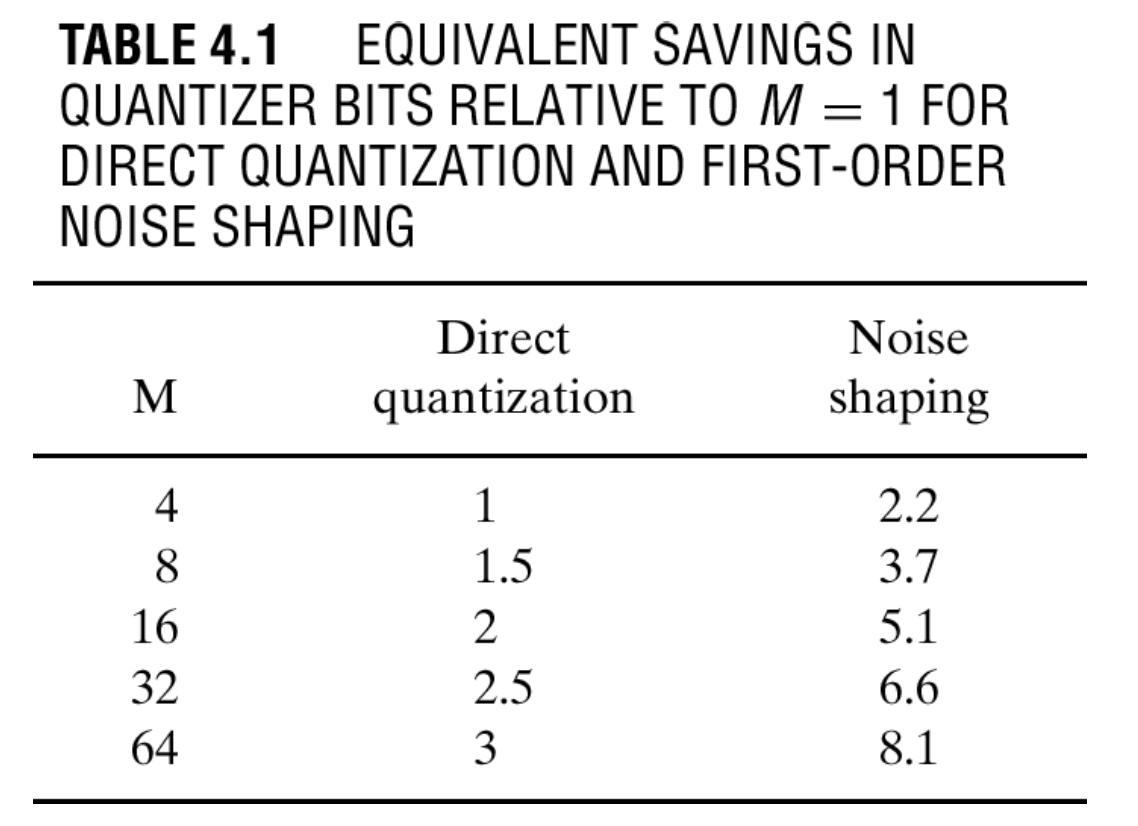
\includegraphics[width=0.9\textwidth]{figs/table41.png}
\end{figure}

\end{frame}


%
\begin{frame}{Summary}
\begin{itemize}
	\item Quantization is unavoidable in DSP systems
	\item Although quantization is a nonlinear operation on a signal, it is a linear operation on the signal PDF (area sampling)
	\item The probabilistic interpretation of quantization allows us to model the quantization error as a uniformly distributed random process (linear noise model)
	\item Using this linear noise model, we simply replace quantizers by noise sources of average power $\sigma_e^2 = \Delta^2/12$
	\item Quantization noise is assumed white (samples are uncorrelated)
	\item Every extra bit of resolution in a quantizer improves the SNR by 6.02 dB
	\item The signal amplitude must be matched to the dynamic range of the quantizer, otherwise there'll be excessive clipping or some bits won't be used
	\item Noise shaping is a strategy that minimizes quantization noise in A-to-D and D-to-A converters. The goal is to shape the quantization noise PSD, so that most of the noise power falls outside the signal band
	\item Noise shaping requires oversampling to minimize noise aliasing
\end{itemize}
\end{frame}

\end{document}
